\section{Implementation and evaluation protocol}
\label{app:protocol}

\paragraph{Optimizer and parameter mask.}
B/2 and L/2 initialize from their corresponding released iMF checkpoint. The
AdamW learning rate is $10^{-6}$ with zero weight decay and $\beta_2=0.95$.
The archived setting \texttt{trainable\_imeanflow\_u\_head\_from: 0}
updates all \texttt{u\_heads} blocks and \texttt{u\_final\_layer} within
\texttt{net}, and any leaves outside \texttt{net}; other generator leaves
remain frozen. The B/2 mask updates 56,700,992 of 88,974,400 parameters;
the L/2 mask updates 100,698,128 of 409,054,224 parameters. These are exact
counts. All adaptation runs use this mask. The main B/2 run uses batch 16
and 6K updates (96K noise--label pairs), whereas L/2 uses batch 4 and 16K
updates (64K pairs). All reported students use raw parameters.

\paragraph{Synthetic data and frozen representations.}
Training uses deterministic noise--label pairs from sample IDs starting at
zero, with training seed 42 and sampling seed 20260831. Labels are drawn
uniformly and independently in the primary runs. No target images, target
latents, real-feature caches, or real-reference moments enter adaptation.
Teacher and student endpoints are decoded using the released iMF codec,
then resized to $224\times224$ with bicubic interpolation for the frozen
ImageNet-22K-pretrained ConvNeXtV2-Tiny global-mean representation.
Teacher features and their RMS normalizer are stop-gradient. Gradients
through the frozen image encoder and VAE still reach the student.
The finite-batch objective and feature normalization are specified in
Appendix~\ref{app:m2o-objective}.

\paragraph{Paired perceptual comparator protocol.}
For the L/2 fixed-$K=4$ setting, two controls retain the released
initialization, independent noise--label IDs, optimizer mask, one-step
inference settings, and zero endpoint, anchor, and hidden-loss weights. The
paired ConvNeXt control uses the same decoded images, $224\times224$
resize, frozen global-mean representation, and stop-gradient teacher RMS as
the distribution arm, replacing only its minibatch kernel with normalized
matched-pair feature MSE. The LPIPS control applies frozen official
LPIPS-VGG v0.1 weights to paired decoded RGB images clipped to $[-1,1]$;
the VAE and LPIPS computation remain differentiable with respect to the
student. On synthetic image pairs, its JAX value and image-input gradient
agree with the official PyTorch implementation within $10^{-8}$ RMS/absolute
error. Teacher-image gradients are stopped. Both controls use unit loss
weight. We record full single-H200 training wall time and separately audit
raw one-NFE FID-50K. For a longer-run equal-time comparison, a checkpoint
is chosen by proximity to the distribution arm's measured training time
before reading that checkpoint's FID.
At 4K updates, distribution matching and paired ConvNeXt score 1.83 and
1.82 after 0.33 hour each, while LPIPS scores 3.58 after 0.32 hour. The
preselected longer comparison uses distribution step16K at 0.9336 hour,
paired ConvNeXt step13K at 0.9167 hour, and LPIPS step14K at 0.9308 hour;
their FID-50K values are 1.72, 2.04, and 3.37. Direct step16K paired
ConvNeXt and LPIPS score 2.06 and 3.40 after 1.0656 and 1.0325 hours. All
six paired evaluations use the same 50K bank; the detailed raw reports and
full precision costs are included in the supplement.

The B/2 paired controls use the primary eight-step teacher and one-step
student settings in Table~\ref{tab:sampler-settings}, batch 16, 6K updates,
and 96K independently labelled noise samples. They retain the primary
initialization, parameter mask, optimizer, and zero endpoint/anchor/hidden
weights, with the same paired feature objectives described above.
Paired ConvNeXt reaches 3.84 FID-50K in 2104 seconds (0.5844 H200-hour);
LPIPS-VGG reaches 5.43 in 2082 seconds (0.5783 H200-hour).
Each completes training in one process, including setup and compilation,
then evaluates raw checkpoint 6000 on the common 50K bank with batch 8.
All logged losses and gradient norms are finite. These are fixed-budget
controls rather than an objective-specific hyperparameter search.

\begin{table}[!b]
\centering
\caption{Primary sampler settings. Scales and interval endpoints are retained
at the precision required for reproduction. $K=1$ students have one
conditional branch and one network evaluation.}
\label{tab:sampler-settings}
\begin{tabular}{lrrrrr}
\toprule
Model/mode & $K$ & Guidance & Interval & Noise scale & Output scale \\
\midrule
B/2 baseline/student & 1 & 7.75 & $[0.38,0.65]$ & 0.975 & 0.975 \\
B/2 self-teacher & 8 & 4.60 & $[0.43,0.65]$ & 1.00 & 1.00 \\
L/2 matched baseline/student & 1 & 5.00 & $[0.40,0.60]$ & 1.00 & 1.00 \\
L/2 matched self-teacher & 4 & 5.00 & $[0.40,0.60]$ & 1.00 & 1.00 \\
\bottomrule
\end{tabular}
\end{table}

\paragraph{Evaluation separation.}
For B/2 and L/2, sampler selection uses a 5,000-sample development bank with seed 20260831
and ID offset 500000. Their FID comparisons
uses 50,000 generated samples, the same seed, offset 700000, and strictly
balanced labels $y={\rm sample\_id}\bmod1000$. Evaluation uses the same
real-reference moments and CPU Inception implementation with float32 feature
export. The latent transform is
$z_{\rm VAE}=z_{\rm normalized}\odot\mathrm{std}+\mathrm{mean}$, with
$\mathrm{mean}=(0.86488,-0.27787,0.21617,0.37384)$ and
$\mathrm{std}=(4.85504,5.31922,3.93725,3.98700)$.
Reference moments are used for post-training evaluation and sampler/model
selection, so dataset-free refers to adaptation rather than the entire
selection pipeline. Repeated development comparisons on the 50K bank do not
constitute an untouched test set. Reports record seeds, ID offsets, codec,
branch count, and NFE. The final and independent 22-file rerun archives are
SHA-256 verified; raw export verifies parameter count and serialization.

\paragraph{Cost boundary.}
B/2 and L/2 adaptation time includes initialization, compilation, online teacher sampling,
VAE decoding, feature extraction, optimization, and checkpointing on one H200. It excludes
checkpoint pretraining, sampler selection, and final evaluation. The recorded
L/2 eight-step sampler search costs 5.17 H200-hours; a five-point four-step
follow-up costs 1.07 H200-hours. These are additional evaluation costs,
not included in the 0.93-hour adaptation claim. The B/2 discovery process
includes earlier experiments whose full search cost is not summarized by
the primary training figure. Therefore we claim low-cost adaptation once a
teacher setting is chosen.
The independent B/2 host rerun uses the same training seed and reaches
3.00 FID-50K in 0.59 H200-hour. Intermediate L/2 checkpoint times in
Figure~\ref{fig:compute-curve} are approximate.

\paragraph{Class fidelity and coverage.}
A frozen ResNet-50V2 checks 50K generated images per arm.
Requested-class top-1 rises from 87.21\% to 87.86\% for B/2 and from
84.91\% to 87.08\% for fixed-guidance L/2. All 1,000 predicted classes
remain covered; within-class feature distances contract slightly.
Table~\ref{tab:diagnostics} reports the full statistics.

\begin{table}[!t]
\centering
\caption{Frozen ResNet-50V2 diagnostics on 50K generated images.
B/2 teacher/student sampler settings differ; L/2 settings are shared.}
\begin{tabular}{lrrr}
\toprule
Arm & Top-1 (\%) & Top-5 (\%) & Within-class distance \\
\midrule
B/2 calibrated baseline & 87.21 & 97.16 & 0.47 \\
B/2 primary student & 87.86 & 97.43 & 0.46 \\
B/2 selected teacher & 86.98 & 97.09 & 0.48 \\
B/2 same-class student & 86.95 & 97.14 & 0.47 \\
\midrule
L/2 same-CFG baseline & 84.91 & 96.51 & 0.51 \\
L/2 primary $K=4$ student & 87.08 & 97.31 & 0.49 \\
L/2 paired ConvNeXt 4K student & 87.87 & 97.72 & 0.48 \\
L/2 $K=4$ teacher & 88.07 & 97.88 & 0.49 \\
L/2 same-class student & 87.66 & 97.61 & 0.49 \\
\bottomrule
\end{tabular}
\label{tab:diagnostics}
\end{table}

\subsection{XL/2 configuration and evaluation}
\label{app:xl-protocol}
The XL/2 result in Table~\ref{tab:model-context} initializes the student and
frozen teacher from the released iMF-XL/2 checkpoint. The same parameter
mask updates 100,698,128 of 610,415,632 generator parameters. Training uses
16,000 AdamW updates with batch size 4 (64,000 generated noise--label pairs),
constant learning rate $10^{-6}$, $\beta_2=0.95$, and zero weight decay.
The training seed is 42 and the generated-pair seed is 20260831, with
uniformly sampled independent labels. The loss is the unit-weight
ConvNeXtV2-Tiny distribution term in Appendix~\ref{app:m2o-objective};
endpoint, anchor, hidden-state, and composition-consistency weights are zero.
The frozen encoder uses bfloat16 computation and global-mean features after
the same $224\times224$ image resize and teacher-RMS normalization.
EMA is maintained with decay 0.999; the reported student uses raw weights.

The teacher uses two uniform steps, $1\!\to\!0.5\!\to\!0$, implemented with
\texttt{lax.scan}, guidance 4.00, and interval $[0.36,0.64]$.
The one-step baseline and student use guidance 8.00 and interval
$[0.42,0.62]$. Input-noise and output scales are both 1.00.
The raw checkpoint at 16K updates is selected using FID-5K from the
predeclared 4K and 16K milestones before final FID-50K evaluation.

XL/2 evaluation follows the upstream iMF seed-99 protocol, using the same
50,000 noise--label pairs for the baseline and student. Noise is generated
in blocks of 80: fold seed 99 by the block index, split the resulting key
three ways, and use the second key for float32 Gaussian noise of shape
$(80,32,32,4)$. Labels cycle through the 1,000 classes. Generator batch size
is 80; VAE decoding and upstream Inception feature extraction use batches
of 8, with FID statistics accumulated in float64. The final evaluation
uses the upstream sampler; the one-step project and upstream outputs agree
exactly in the checked latent batch. This protocol yields FID-50K 1.70 for
the released baseline and 1.62 for the selected student. The B/2 and L/2
results retain their evaluation bank described above.

\section{Additional controls and interpretation}
\label{app:controls}

\paragraph{Endpoint and initialization controls.}
The B/2 endpoint-only arm uses latent MSE weight 0.1 and reaches 17.69
FID-50K in 0.23 H200-hour; adding a one-step anchor of weight 1.0 reaches
3.35 in 0.22 hour. The L/2 $K=4$ endpoint-only arm instead uses weight 1.0
and reaches 13.33 in 0.67 hour. The endpoint-plus-
distribution arms use endpoint weight 0.1. Randomizing only the trainable
B/2 leaves while retaining the frozen pretrained leaves yields 346.03
FID-50K in 0.62 hour with endpoint-plus-distribution training. This failure
supports the importance of the pretrained initialization in this short
adaptation regime.

\paragraph{Hidden alignment.}
The B/2 matched pair augments endpoint-plus-distribution training with sparse
readouts at student layers 2, 5, and 8 and teacher rollout states 2, 4, and 6.
A normalized latent MSE coefficient of 0.001 reduces the final hidden loss
from 0.96 to 0.77; both aligned and zero-weight arms score 3.05 FID-50K.
The zero-weight arm computes the same readouts. Both arms use the
endpoint-plus-distribution recipe.

\paragraph{Exploratory class grouping.}
The primary independent-label batches mainly compare images across classes.
A subsequent same-class minibatch variant reaches B/2 FID-50K 3.05, 2.94,
and 2.87 after 1K, 3K, and 6K updates, with costs 0.16, 0.33, and 0.59
H200-hour. A same-host independent-label 6K run reaches 3.00 in 0.59 hour.
For L/2 at fixed $K=4$, same-class training reaches 1.69 in 0.92 hour versus
the primary 1.72. A round-robin cross-class arm reaches 1.75, and regrouping
the same pair set into cross-class batches reaches 1.72, both in 0.92 hour.
Batch composition changes the finite-batch objective and optimization order.
Independent-label runs remain primary.

\paragraph{Paired endpoint objectives.}
Let $G_0$ be the frozen released one-step endpoint. The B/2 paired baseline is
\begin{equation}
\mathcal L_{\rm endpoint}
=0.1\,\mathbb E\|G_\theta-T_K\|_2^2
+\lambda_0\,\mathbb E\|G_\theta-G_0\|_2^2,
\label{eq:endpoint}
\end{equation}
using elementwise mean reductions, with $\lambda_0=0$ or $1$.
The L/2 endpoint-only control uses unit endpoint weight as specified above.
The primary M2O objective contains neither endpoint nor anchor terms.

\paragraph{Additional sampler controls.}
The B/2 two-step control uses the primary teacher settings
(CFG=4.60, interval $[0.43,0.65]$) and student settings
(CFG=7.75, interval $[0.38,0.65]$, input/output scales 0.975).
It retains the 6K-update, batch-16 budget and distribution-only objective.
The teacher scores 2.89237 FID-50K; the student scores 3.06520 after
1783 seconds (0.4953 H200-hour), including setup and compilation.
Reports and the verified source snapshot are in
\texttt{evidence/b2\_k2/} in the supplement.

In an exploratory B/2 same-CFG comparison, the released one-step baseline
scores 4.06, one-step self-matching scores 4.04, and eight-step-to-one
adaptation reaches 2.86 after 0.61 H200-hour. The student configs differ only
in teacher step count. Extending the latter to 12K updates gives 2.89 in
1.10 hours. The main tables use the primary selected-sampler settings.
The L/2 step-count comparison fixes guidance and all other sampling settings
as reported in Table~\ref{tab:compute-teacher}.

\clearpage
\section{M2O objective details}
\label{app:m2o-objective}
For feature dimension $d_\phi$ and batch size $n$, the common teacher RMS is
\begin{equation}
c=\operatorname{sg}\!\left[
\left(\frac{1}{n d_\phi}\sum_{i,j}t_{ij}^{2}+10^{-6}\right)^{1/2}
\right],\qquad
\tilde s_i=s_i/c,\quad \tilde t_i=t_i/c.
\end{equation}
The primary recipe uses Equation~\ref{eq:dist} with unit weight and zero
endpoint, anchor, and hidden-state weights. Its KID-style objective uses
ConvNeXt features, batch-dependent teacher normalization, and exclusion of
the paired cross diagonal. The finite-batch surrogate can be negative;
the batch-dependent normalization differs from a fixed-population MMD
estimator. Independent-label batches predominantly contain cross-class
off-diagonal pairs. The pretrained initialization carries the class structure,
which is evaluated by the classifier diagnostics in Table~\ref{tab:diagnostics}.

Figure~\ref{fig:m2o-objective} illustrates the generated-distribution objective
in Section~\ref{sec:method}. It uses $u_i=\tilde s_i=s_i/c$ and
$v_i=\tilde t_i=t_i/c$ to keep the normalized-feature notation compact.
The paired teacher and student endpoints share sample IDs, and their
cross-term contributions use different IDs. The student receives gradients through
the frozen VAE and visual encoder; the teacher features and common RMS scale
are stop-gradient.

\begin{figure}[h]
\centering
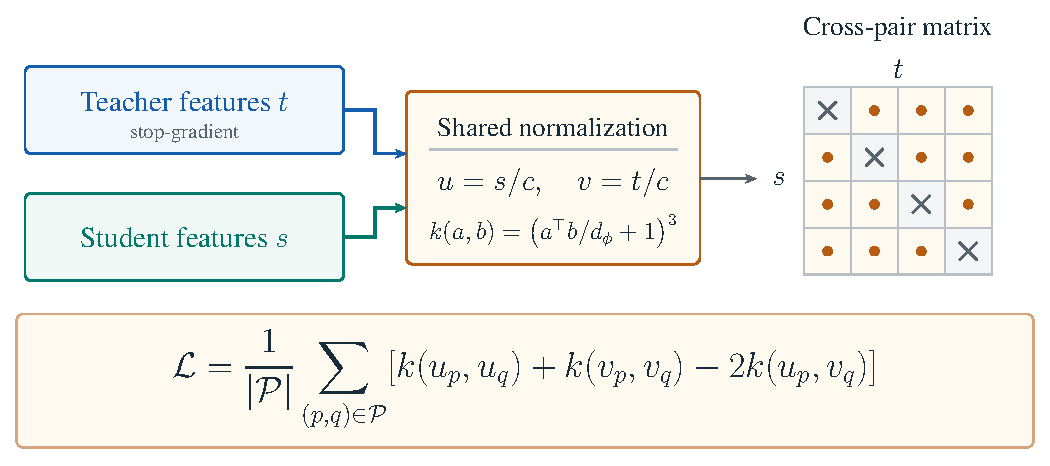
\includegraphics[width=\linewidth]{figures/m2o_objective.pdf}
\caption{M2O's KID-style distribution objective. The cubic kernel compares
normalized global features across a minibatch, excluding self diagonals and
the paired teacher--student cross diagonal. Here
$\mathcal P=\{(p,q):1\le p,q\le n,\ p\ne q\}$, so $|\mathcal P|=n(n-1)$.
The $4\times4$ matrix illustrates the cross-term index mask, with student
rows and teacher columns; crosses are excluded and dots retained.
B/2 uses batch 16 and L/2 batch 4. The common RMS
normalizer is computed from the teacher batch; $d_\phi$ denotes the feature
dimension, as in Equation~\ref{eq:dist}. Both branches use the same frozen encoder; the student
branch backpropagates through it to selected generator parameters. The primary
recipe uses only this distribution term.}
\label{fig:m2o-objective}
\end{figure}

\section{Limitations and further directions}
\label{app:scope}
The controlled experiments cover B/2 and L/2 on ImageNet-256, with an
additional XL/2 result and one training seed per key arm.
B/2 and XL/2 use selected teacher/student guidance; L/2 uses
fixed guidance. The ConvNeXtV2 encoder is pretrained on ImageNet-22K;
its visual prior is therefore derived from the same broader ImageNet
collection as the ImageNet-1K benchmark. Pretrained iMF and VAE weights
also supply image-derived prior knowledge. Dataset-free describes access
during adaptation. Real-reference moments enter evaluation
and model selection, with compute accounting given in
Appendix~\ref{app:protocol}. Further directions include broader model
families, full-model adaptation, independent training seeds, and
real-reference diversity evaluation. Classifier agreement and predicted-class
coverage measure conditional fidelity but do not establish real-distribution
coverage. The L/2 recipe uses four images per update; an equal-budget
batch-size study and repeated-seed estimates of the finite-batch objective
remain open. Direct comparisons with alternative distillation methods
and continued iMF training would further characterize how to allocate a
small adaptation budget; original iMF training would require a different,
real-data-access protocol.


\section{Complete shared-noise qualitative comparisons}
\label{app:qualitative}
Figures~\ref{fig:qualitative-full-b2} and~\ref{fig:qualitative-full-l2}
show all eight examples declared before rendering. Every column shares
the same noise and class label across baseline, teacher, and student.
The raw checkpoint, config, source, and image hashes are archived in
\texttt{evidence/fixed\_id\_grids/}. The original images are preserved
without retouching; the main-text panels use identical crop coordinates
across rows, recorded in \texttt{figures/qualitative\_selection.json}.
The main text selects four full-image cases and three detail cases after
inspecting these grids. Full-image panels retain the complete image extent;
the detail panels use the matched regions recorded in the selection file.
B/2 uses its primary eight-step teacher and student settings. L/2 uses
the primary four-step-teacher student trained for 0.93 H200-hour, with
CFG=5.00 for all three rows.

\begin{figure}[htbp]
\centering
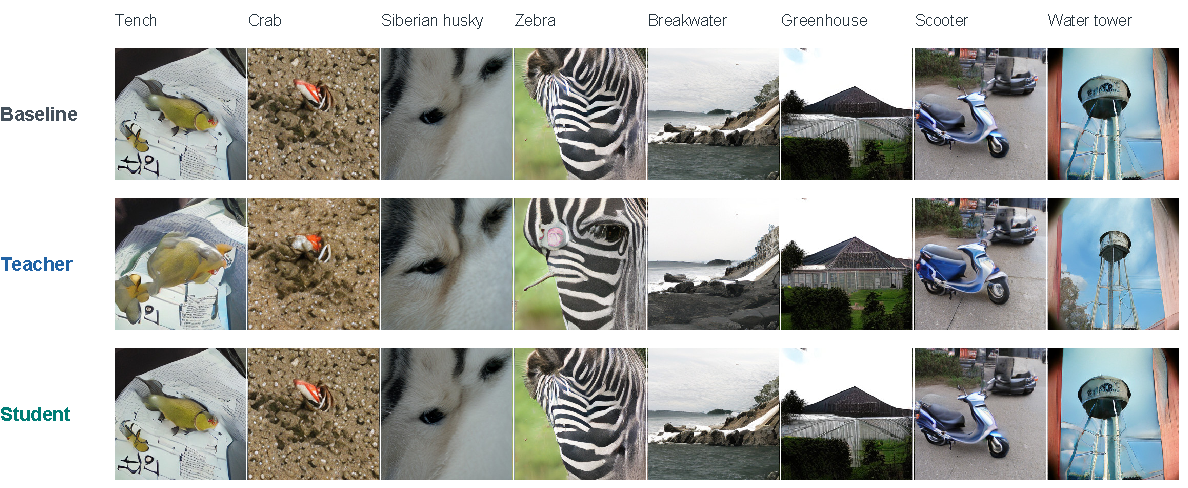
\includegraphics[width=\linewidth]{figures/qualitative_full_b2.pdf}
\caption{Complete predeclared B/2 bank. Rows: released one-step baseline,
frozen eight-step self-teacher, and primary one-step M2O student.
Teacher and student use their respective primary sampling settings.}
\label{fig:qualitative-full-b2}
\bigskip
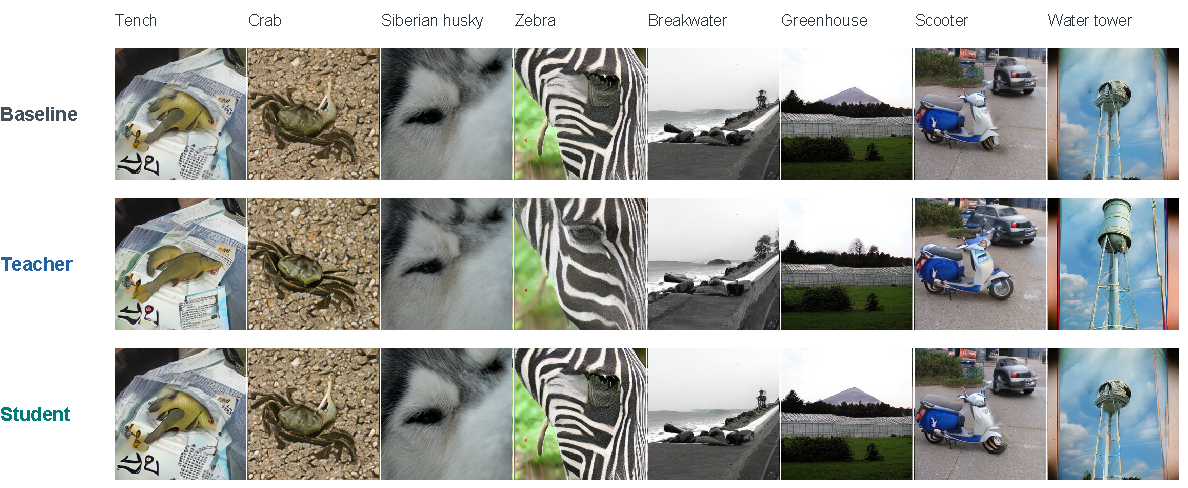
\includegraphics[width=\linewidth]{figures/qualitative_full_l2.pdf}
\caption{Complete predeclared L/2 bank. Rows: released one-step baseline,
frozen four-step self-teacher, and primary one-step M2O student
(0.93 H200-hour). All rows use fixed CFG=5.00, the same guidance interval,
and unit input/output scales.}
\label{fig:qualitative-full-l2}
\end{figure}

\clearpage
\section{Uncurated one-step samples}
\label{app:uncurated}
Figures~\ref{fig:uncurated-b2} and~\ref{fig:uncurated-l2} show 128 uncurated
samples from the primary M2O students. Each row contains the first eight
evaluation samples for a class chosen before generation. All samples are
shown in order, using the primary settings in Table~\ref{tab:sampler-settings}.

\begin{figure}[htbp]
\centering
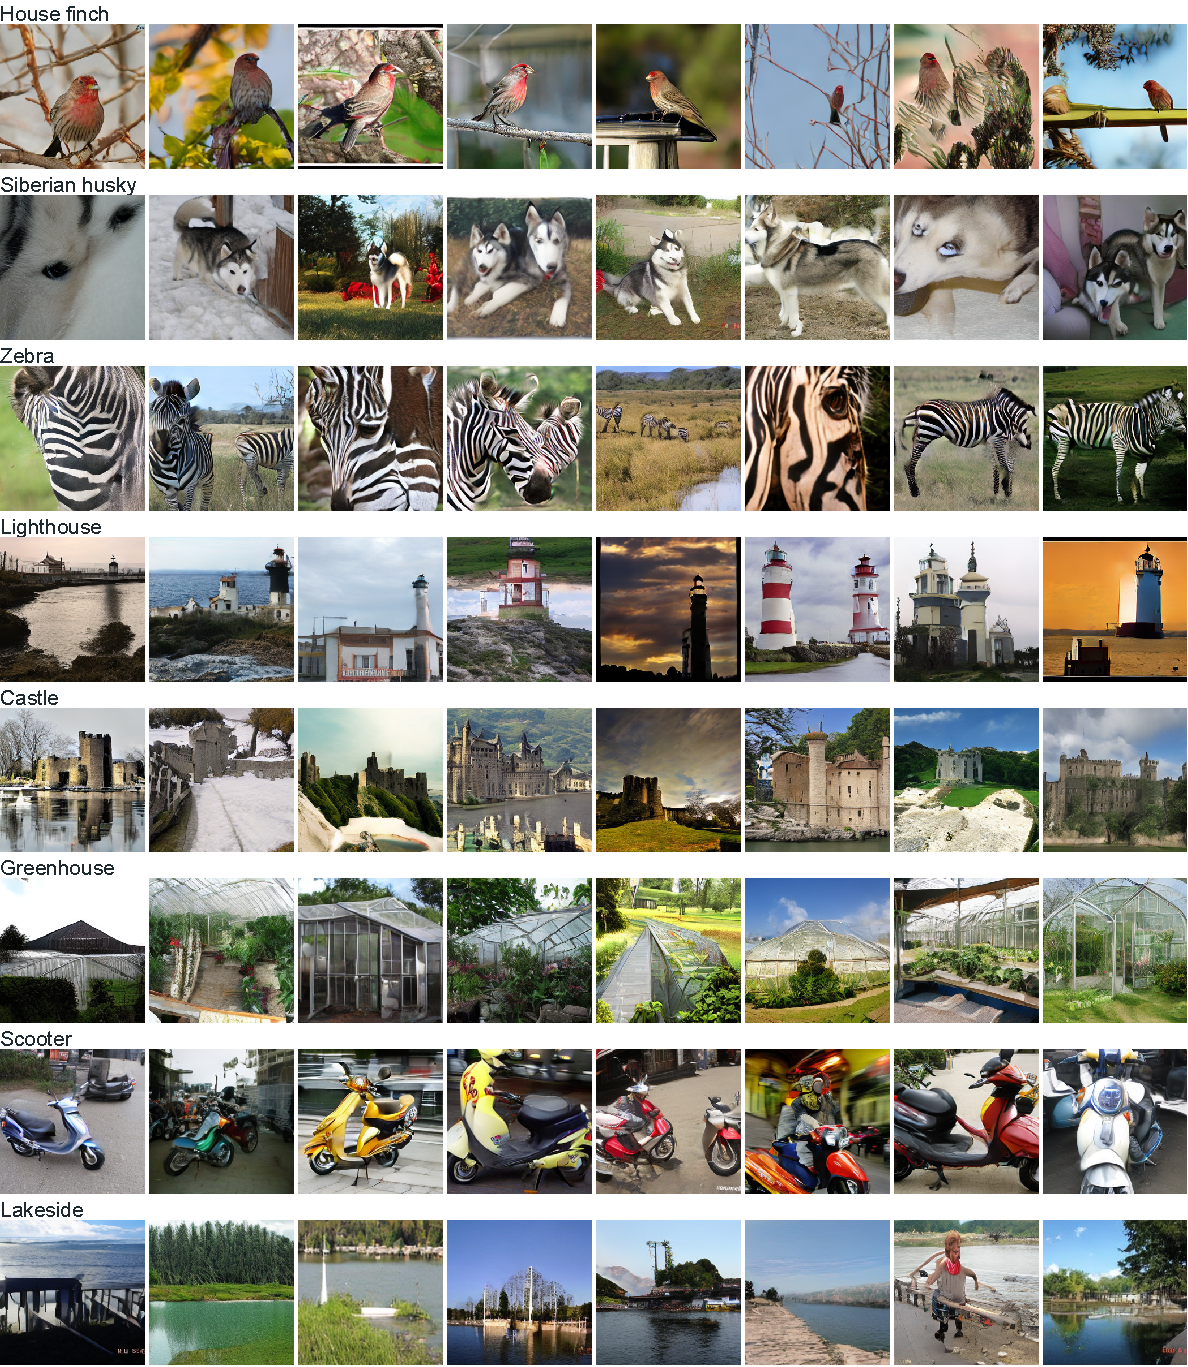
\includegraphics[width=\linewidth]{figures/uncurated_b2.pdf}
\caption{Uncurated one-step generation from iMF-B/2 + M2O
(FID-50K 3.00; 0.60 H200-hour adaptation). Each row shows eight samples
of the indicated class, with complete images and no sample filtering.}
\label{fig:uncurated-b2}
\end{figure}

\clearpage
\begin{figure}[t]
\centering
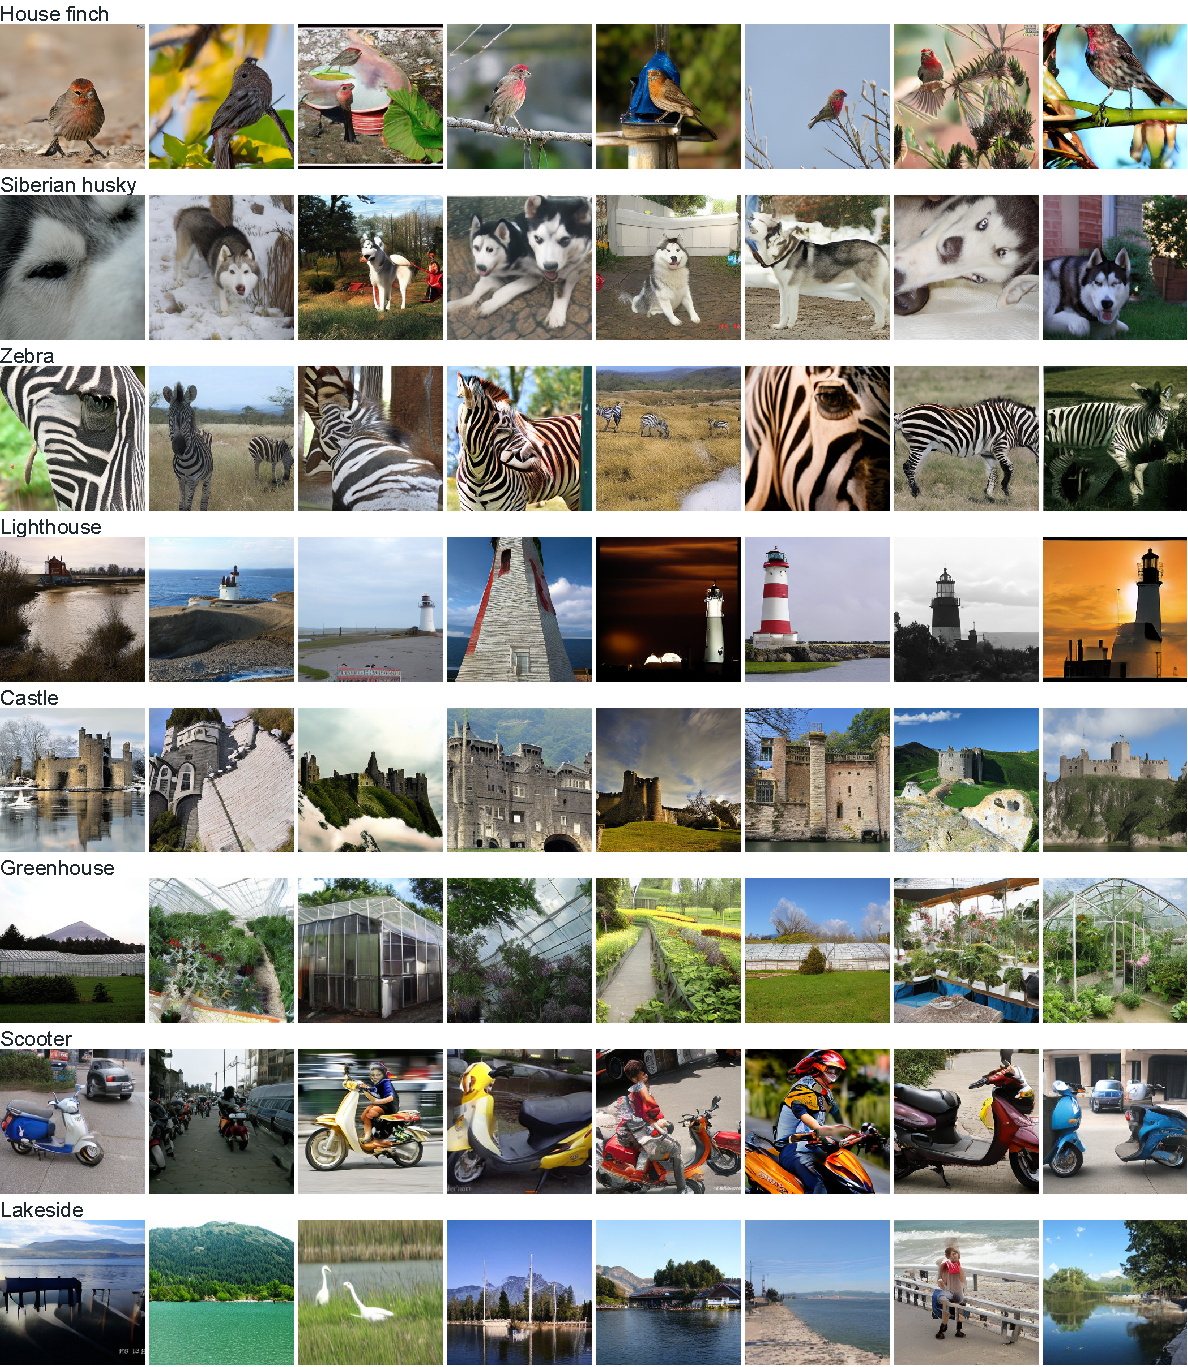
\includegraphics[width=\linewidth]{figures/uncurated_l2.pdf}
\caption{Uncurated one-step generation from iMF-L/2 + M2O
(FID-50K 1.72; 0.93 H200-hour adaptation). Class order and noise IDs match
Figure~\ref{fig:uncurated-b2}. The primary four-step-teacher student uses
CFG=5.00; all eight samples per class are shown without filtering.}
\label{fig:uncurated-l2}
\end{figure}
